\section{Theoretical Analysis}
\label{sec:analysis}

In this section, the circuit shown in Figure~\ref{fig:Circuit_Base} is analyzed theoretically with the Nodal Method and General Solution Method in order to caracterize it in the interval $\left[-5,20\right[$.

\subsection{Step 1: Solution for $t<0$}

When $t<0$ we consider that the circuit is in equilibrium and, because of that, no current passes through the capacitor, since the relation between current and voltage in this component is:
\begin{equation}
  \frec{dV}{dt}=\frac{I}{C} \rightarrow I = 0.
  \label{eq:Cap}
\end{equation}

Hence, we can simplify the circuit:
\begin{figure}[h] \centering
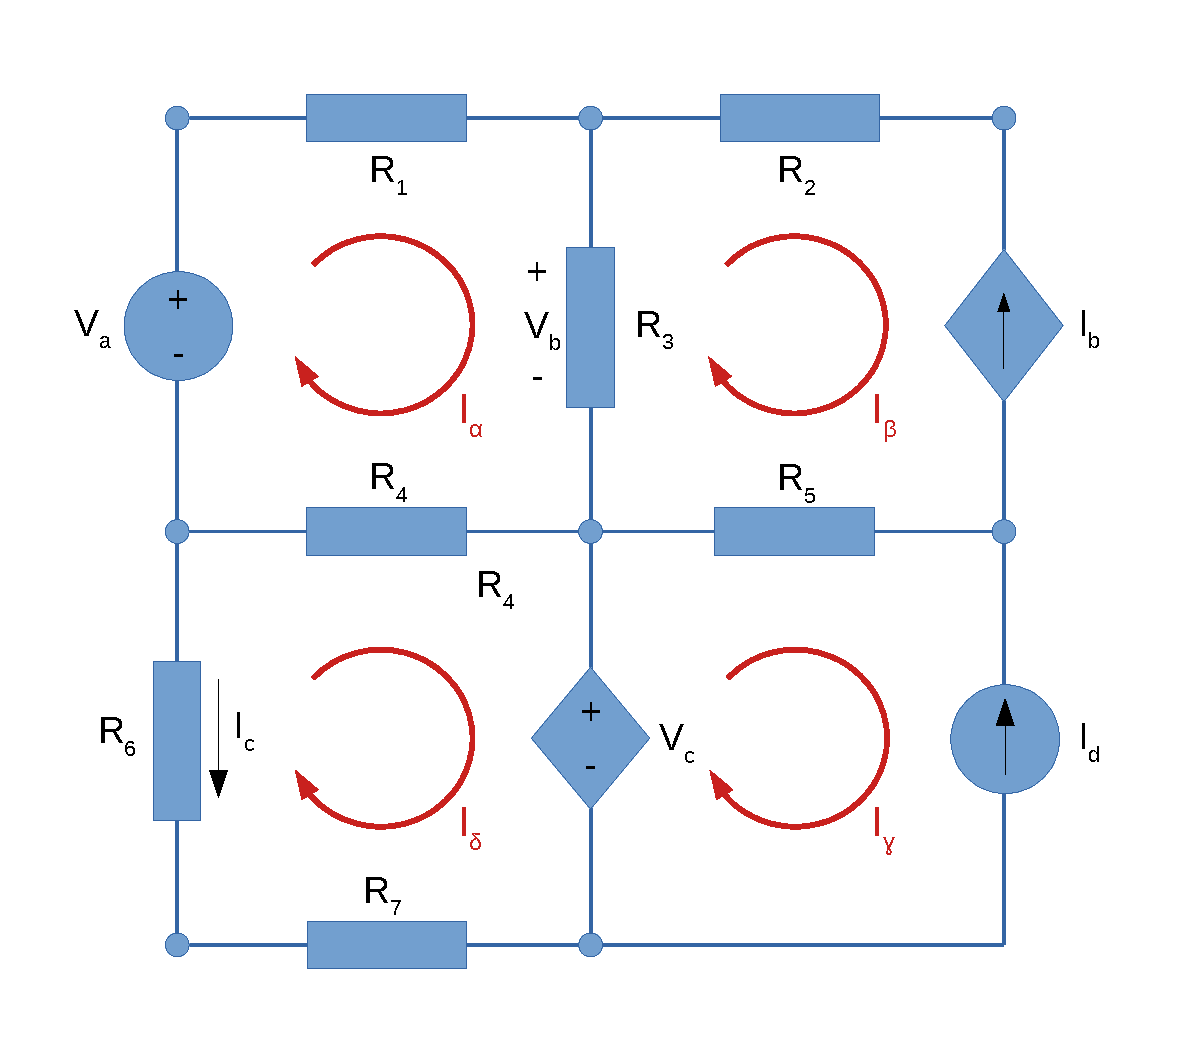
\includegraphics[width=0.45\linewidth]{CircuitMesh.pdf}
\caption{Circuit analysed with mesh currents.}
\label{fig:Circuit_Passo1}
\end{figure}

Applying the Nodal Method to this circuit leads to the following equations:

\begin{equation}
\begin{cases}
	v_1 - v_4 &= V_s;																				  \\
	\frac{1}{R_1}v_1 - (\frac{1}{R_2}+\frac{1}{R_1}+\frac{1}{R_3})v_2 + (\frac{1}{R_2})v_3 + \frac{1}{R_3}v_5 &= 0; 																						  \\
  	\frac{1}{R_2}v_2 - \frac{1}{R_2}v_3+ I_b &= 0;													  \\
  	-\frac{1}{R_1}v_1 + \frac{1}{R_1}v_2 - (\frac{1}{R_4}+\frac{1}{R_6})v_4 + \frac{1}{R_4}v_5 + \frac{1}{R_6}v_7 &= 0;			  																	  \\
	v_5 - v_8 - V_d &= 0;																			  \\
  	\frac{1}{R_5}v_5 - \frac{1}{R_5}v_6 - I_b &= 0;												  	  \\
  	-(\frac{1}{R_7}+\frac{1}{R_6})v_7 + \frac{1}{R_7}v_8 + \frac{1}{R_6}v_4 &= 0;					  \\
	v_2 - v_3 - V_b &= 0;																			  \\
  	\frac{1}{R_6}v_4 - \frac{1}{R_6}v_7 - I_d &= 0;													  \\
  	v_4 &= 0;																						  \\
  	-K_bV_b + I_b &= 0;																				  \\
  	V_d - K_cI_c &= 0.
\end{cases}
\end{equation}

Where the $2^{nd}$, $3^{rd}$, $6^{th}$ and $7^{th}$ are the equations in the respective nodes; the $1^{st}$ and $5^{th}$ are the relations imposed by the voltages soureces in those nodes; the $4^{th}$ is the supernode that bypasses $V_s$; the $8^{th}$ to $10^{th}$ are the relations between the circuit and, in order, $V_b$, $I_d$ and $v_4$; the final two equations are the ones that describe $I_b$ and $V_d$, respectivly. 
The solution to this linear system of equations is determined by Octave, plus the currents flowing in the circuit using Ohm's Law to the resistor's branches and Kirchhoff Current Law~(KCL) to the branches with voltage sources:

\begin{table}[h]
  \centering
  \begin{tabular}{|l|r|}
    \hline    
    {\bf Name} & {\bf Value [A or V]} \\ \hline
    \input{../mat/PASSO1_tab}
  \end{tabular}
  \caption{Variables in the Mesh Method. A variable preceded by @ is of type {\em current} and expressed in Ampere; other variables are of type {\em voltage} and expressed in Volt.}
  \label{tab:PASSO1}
\end{table}

All the currents were measured from the lower numbered node to the higher one; so, the direction of the current that passes through $R_6$ is, if the result is positive, from $v_4$ to $v_7$.

\subsection{Step 2: Solution for $t=0$ and $R_{eq}$}

Once found the solution for the nodes in $t<0$, the next step is to calculate the boundary conditions for the knots in the circuit, because the voltage in the nodes doesn't necessarily need to be continuos, only the difference of potencial in the capacitor, $V_c$. Therefor, a non continuos change in a power source, in this case in the voltage source $V_s$, might lead to a diferent voltage in the nodes.
Since the solution to this circuit will also be divided in natural and forced, we can use this step to evaluate the equivelent resistance of the circuit, $R_{eq}$.

To evaluate the circuit at $t=0$, we must have in mind that $V_c$ is continuos, so $V_c(0)=V_c(0^-)$. Another point to take into account is that, for the natural solution, we can ignore the sinusoidal part of $V_s$, which leaves us with $V_s=0$. In this conditions, we can say that the circuit~\ref{fig:Circuit_Base} is identical to this one:

\begin{figure}[h] \centering
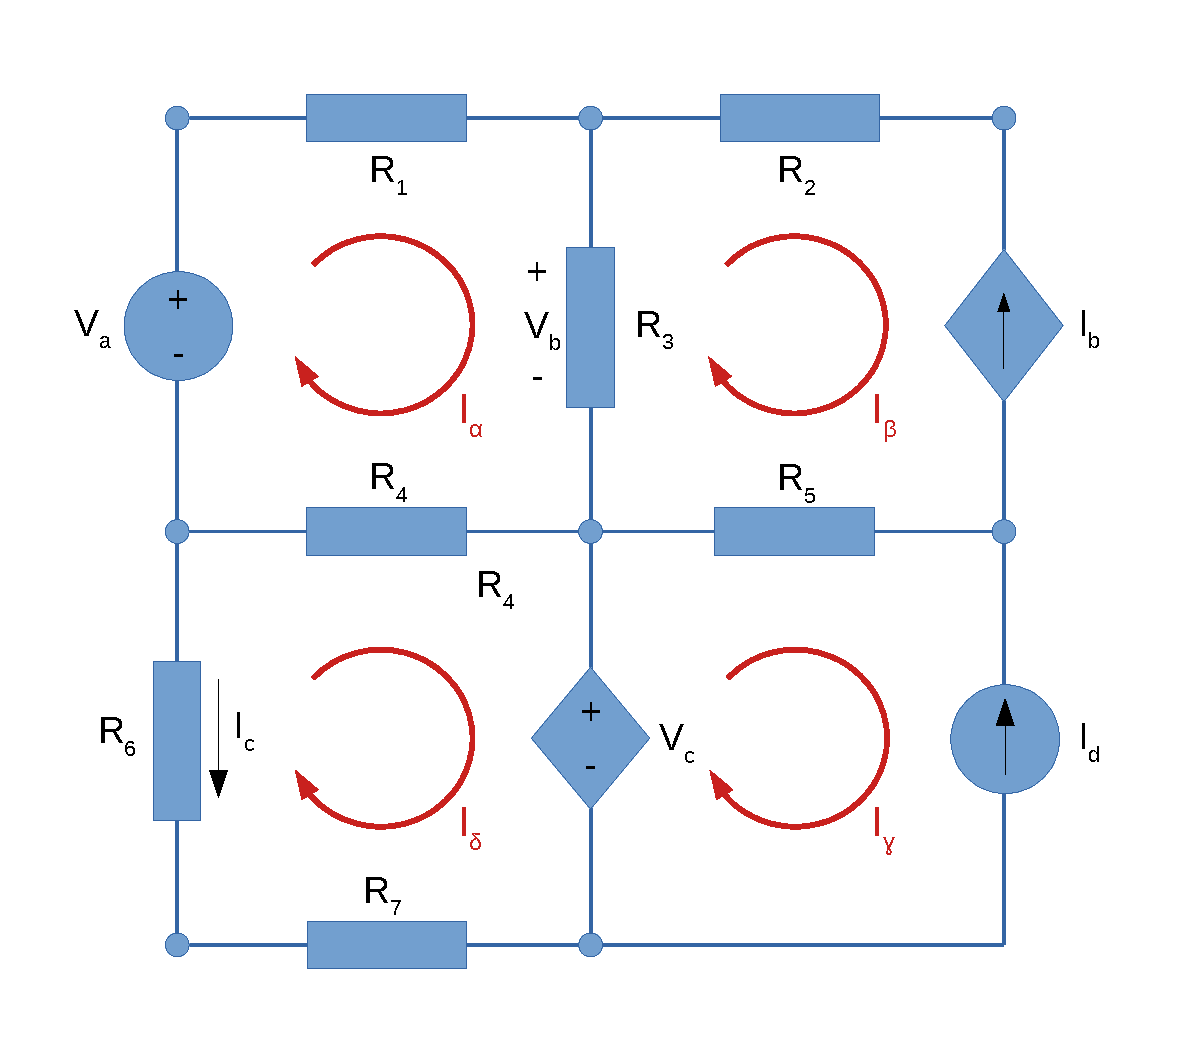
\includegraphics[width=0.45\linewidth]{CircuitMesh.pdf}
\caption{Circuit analysed with mesh currents.}
\label{fig:Circuit_Passo2}
\end{figure}

The set of equations that describe it are, using the Nodal Method:

\begin{equation}
\begin{cases}
	v_1 - v_4 &= 0;																				  \\
	\frac{1}{R_1}v_1 - (\frac{1}{R_2}+\frac{1}{R_1}+\frac{1}{R_3})v_2 + (\frac{1}{R_2})v_3 + \frac{1}{R_3}v_5 &= 0; \\
  	\frac{1}{R_2}v_2 - \frac{1}{R_2}v_3+ I_b &= 0;													  \\
  	-\frac{1}{R_1}v_1 + \frac{1}{R_1}v_2 - (\frac{1}{R_4}+\frac{1}{R_6})v_4 + \frac{1}{R_4}v_5 + \frac{1}{R_6}v_7 &= 0;			  																	  \\
	v_5 - v_8 - V_d &= 0;																			  \\
  	\frac{1}{R_5}v_5 - \frac{1}{R_5}v_6 - I_b &= 0;												  	  \\
  	-(\frac{1}{R_7}+\frac{1}{R_6})v_7 + \frac{1}{R_7}v_8 + \frac{1}{R_6}v_4 &= 0;					  \\
	v_2 - v_3 - V_b &= 0;																			  \\
  	\frac{1}{R_6}v_4 - \frac{1}{R_6}v_7 - I_d &= 0;													  \\
  	v_4 &= 0;																						  \\
  	-K_bV_b + I_b &= 0;																				  \\
  	V_d - K_cI_c &= 0.
\end{cases}
\end{equation}



\subsection{Nodal Method}

Firstly, computing the values of current and voltage using the nodal method requires finding all the knots in the circuit, as it is presented in Figure \ref{fig:Circuit_Nodal}.
\begin{figure}[h] \centering
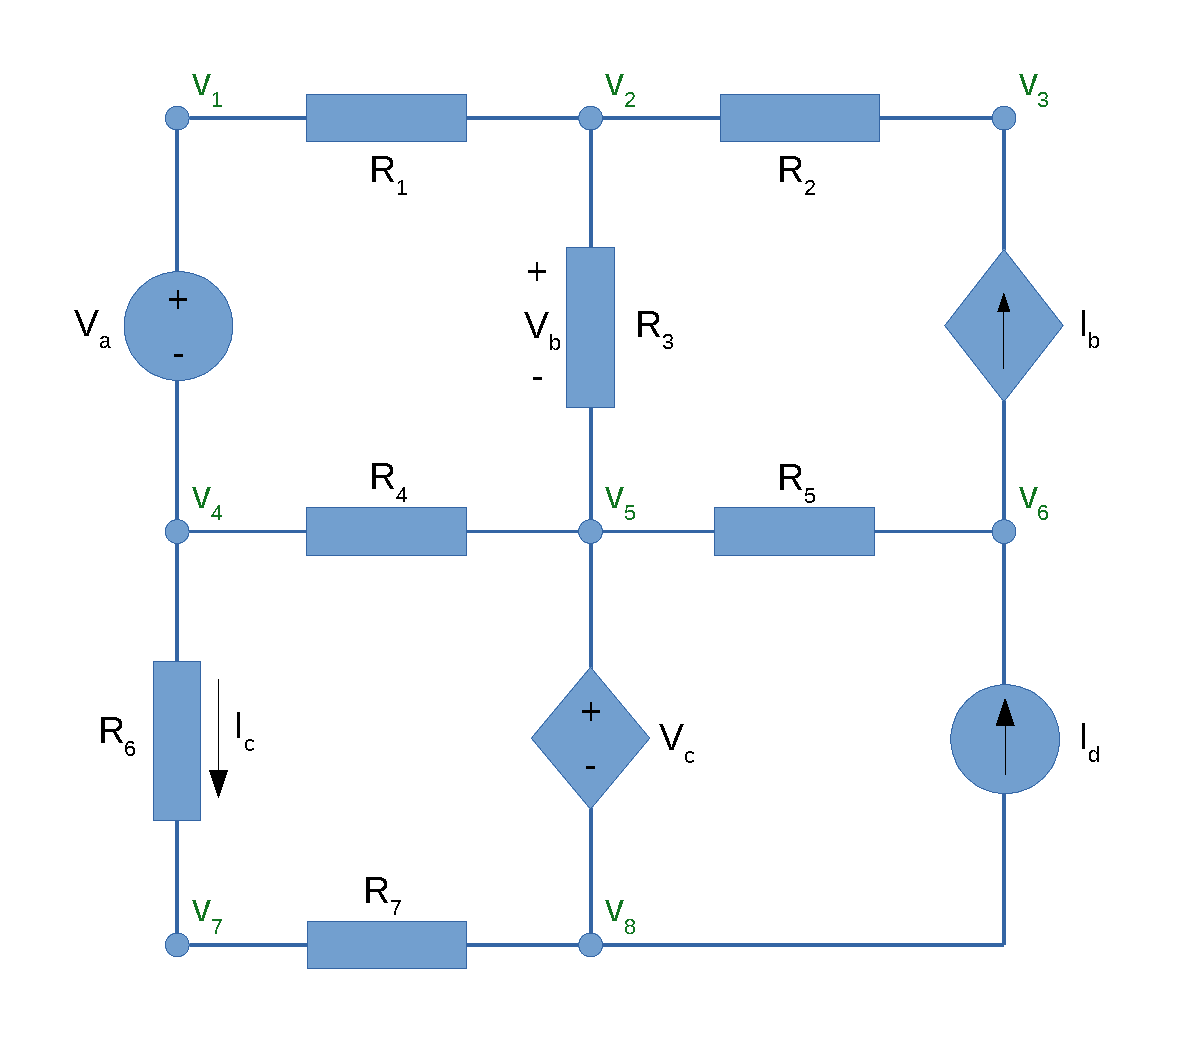
\includegraphics[width=0.5\linewidth]{CircuitNodal.pdf}
\caption{Circuit analysed with nodal voltages.}
\label{fig:Circuit_Nodal}
\end{figure}

Then, the Kirchhoff Current Law~(KCL) is used in the nodes not connected to voltage sources (Equations~\ref{eq:NM_Point2}~to~\ref{eq:NM_Point7}) and two additional equations relating the knots voltages with the voltage sources connected to them are presented (Equations~\ref{eq:NM_Va}~and~\ref{eq:NM_Vc}):

\begin{equation}
  \frac{v_3-v_2}{R_2} + \frac{v_2-v_5}{R_3} + \frac{v_1-v_2}{R_1} = 0;
  \label{eq:NM_Point2}
\end{equation}
\begin{equation}
  I_b + \frac{v_2-v_3}{R_2} = 0;	
  \label{eq:NM_Point3}
\end{equation}
\begin{equation}
  \frac{v_5-v_6}{R_5} - I_b + I_d = 0;
  \label{eq:NM_Point6}
\end{equation}
\begin{equation}
  \frac{v_4-v_7}{R_6} + \frac{v_8-v_7}{R_7} = 0;
  \label{eq:NM_Point7}
\end{equation}

\begin{equation}
  v_1 - v_4 = V_a;
  \label{eq:NM_Va}
\end{equation}
\begin{equation}
  v_5 - v_8 = V_c.
  \label{eq:NM_Vc}
\end{equation}

Since there are 8+4 variables ($v_1$~to~$v_8$, $V_b$, $V_c$, $I_b$, $I_c$), the system is defined by twelve independent equations. Two are provided in the circuit and are the same as in the Mesh Method, (\ref{eq:Vb_Ib})~and~(\ref{eq:Vc_Ic}).
By observing the circuit,
\begin{equation}
  v_2 - v_5 = V_b.
  \label{eq:NM_Vb}
\end{equation}

Using Ohm’s Law, the following relation is found:
\begin{equation}
  \frac{v_4-v_7}{R_6} = I_c.
  \label{eq:NM_OhmIc}
\end{equation}

Because there needs to be a knot with a defined voltage, we chose $v_4$ to be connected to the ground:
\begin{equation}
  v_4 = 0.
  \label{eq:NM_v4=0}
\end{equation}

For the last equation, the continuity of current in the circuit can be used to create a “super-knot”, bypassing the voltage sources $V_a$ and $V_c$, from which the equations are~(\ref{eq:NM_SPVa}) and~(\ref{eq:NM_SPVc}), respectively:

\begin{equation}
  \frac{v_5-v_4}{R_4} + \frac{v_2-v_1}{R_1} - \frac{v_4-v_7}{R_6} = 0;
  \label{eq:NM_SPVa}
\end{equation}
\begin{equation}
  \frac{v_7-v_8}{R_7} - Id + \frac{v_6-v_5}{R_5} + \frac{v_2-v_5}{R_3} + \frac{v_4-v_5}{R_4} = 0.
  \label{eq:NM_SPVc}
\end{equation}

Given that only one more equation is needed, we chose to use the simpler one~(\ref{eq:NM_SPVa}).
%	IMPORTANTE VER OS NÓS
%	AS PRIMEIRAS 7 EQUAÇÕES SÃO DOS NÓS 1 A 7, EM QUE O PRIMEIRO NÓ COM UMA FONTE DE TENSÃO MOSTRA A RELAÇÃO ENTRE OS NÓS EXTREMOS, A SEGUNDA (DO OUTRO NÓ) FAZ A EQUAÇÃO DO SUPERNÓ
%	AS EQUAÇÕES 8 E 9 SÃO AS RELAÇÕES NO CIRCUITO COM AS FONTES LINEARES
%	A EQUAÇÃO 10 É O ZERO DOS NÓS
%	AS EQUAÇÕES 11 E 12 SÃO AS RELAÇÕES QUE EXISTEM NAS FONTES LINEARES 

\begin{equation}
\begin{cases}
	v_1 - v_4 &= V_a;																				  \\
	\frac{1}{R_1}v_1 - (\frac{1}{R_2}+\frac{1}{R_1}+\frac{1}{R_3})v_2 + (\frac{1}{R_2})v_3 + \frac{1}{R_3}v_5 &= 0; \\
  	\frac{1}{R_2}v_2 - \frac{1}{R_2}v_3+ I_b &= 0;													  \\
  	-\frac{1}{R_1}v_1 + \frac{1}{R_1}v_2 - (\frac{1}{R_4}+\frac{1}{R_6})v_4 + \frac{1}{R_4}v_5 + \frac{1}{R_6}v_7 &= 0;			  																	  \\
	v_5 - v_8 - V_c &= 0;																			  \\
  	\frac{1}{R_5}v_5 - \frac{1}{R_5}v_6 - I_b &= -I_d;												  \\
  	-(\frac{1}{R_7}+\frac{1}{R_6})v_7 + \frac{1}{R_7}v_8 + \frac{1}{R_6}v_4 &= 0;					  \\
	v_2 - v_3 - V_b &= 0;																			  \\
  	\frac{1}{R_6}v_4 - \frac{1}{R_6}v_7 - I_c &= 0;													  \\
  	v_4 &= 0;																						  \\
  	-K_bV_b + I_b &= 0;																				  \\
  	V_c - K_cI_c &= 0.
\end{cases}
\end{equation}

The solution to this linear system of equations is determined by Octave:

\begin{table}[h]
  \centering
  \begin{tabular}{|l|r|}
  \hline  
    {\bf Name} & {\bf Value [A or V]} \\ \hline
    \input{../mat/Nos_tab}
  \end{tabular}
  \caption{Variables in the Nodal Method. A variable preceded by @ is of type {\em current} and expressed in Ampere; other variables are of type {\em voltage} and expressed in Volt.}
  \label{tab:nos}
\end{table}

